%        File: WeeklyResearchReport_4_19_21.tex
%     Created: Mon Apr 19 08:00 AM 2021 E
% Last Change: Mon Apr 19 08:00 AM 2021 E
%
\documentclass[a4paper]{article}
\usepackage{mathtools}
\usepackage{verbatim}
\usepackage{graphicx}
\usepackage{tabularx}
\usepackage{pgfplots}
\usepackage{adjustbox}
\usepackage{booktabs}
\makeatletter
\let\latex@xfloat=\@xfloat
\def\@xfloat #1[#2]{%
    \latex@xfloat #1[#2]%
    \def\baselinestretch{1}
    \@normalsize\normalsize
    \normalsize
}
\makeatother
\usepackage{amsmath}
\usepackage{mathtools}
\usepackage{epigraph}
\usepackage{cancel}
\usepackage{xcolor}
\newcommand\Ccancel[2][black]{\renewcommand\CancelColor{\color{#1}}\cancel{#2}}
\usepackage{algorithm}
\usepackage{graphicx}
\usepackage[noend]{algpseudocode}
\usepackage{gnuplot-lua-tikz}
\usepackage[utf8]{inputenc}
\usepackage{pgfplots}
\usepackage{tabularx}
\usepackage{hyperref}
\DeclareUnicodeCharacter{2212}{−}
\usepgfplotslibrary{groupplots,dateplot}
\usetikzlibrary{patterns,shapes.arrows}
\pgfplotsset{compat=newest}
\begin{document}
\begin{titlepage}

    \title{
    Daily Research Report}

    \author{ Jeffrey Severino \\
        University of Toledo \\
        Toledo, OH  43606 \\
    email: jseveri@rockets.utoledo.edu}


    \maketitle

\end{titlepage}
\section{Current Research Direction}
\section{Research Performed}

\subsection{Results}
Figure \ref{fig:1} shows the manufactured solution for the mean flow profile. 
The tangent summation method (TSM) was used to generate the axial mach number and 
for the speed of sound.   The tangential mach number was then numerically approximated by 
using the composite trapezoidal rule. The manufactured mean flow profile 
is unique in that it has been generated solely for the verification of swirl 
and does not have physical significance. The ``kinks'' in the solution will allow
there to be a significant magnitude for the derivatives of these solution. 

The TSM was also used to generate the manufactured solutions for the perturbation
variables in Figures \ref{fig:1a}-\ref{fig:4a}. The boundary condition values of 
the MS for $\bar{v}_r$ $dP/dr$ must reflect the actual boundary conditions in SWIRL. 
This is set by using a fairing function. Note that the hard wall condition requires
$\bar{v}_r$ to be zero which is shown in Figure \ref{fig:1a}. While the boundaries for the 
pressure perturbation may not be known, the boundary condition is set with the 
derivative of the pressure perturbation, which may or may not be zero depending
if there is liner for the test case. This is why these functions no longer resemble
tangent function, but in essence still are. 

The results from the numerical integration is presented in Figure \ref{fig:5}. Although 
the slope of the line appears linear, the TSM was still used to generate the 
MS for the speed of sound. To demonstrate the effect of using denser grids, the 
difference between the expected speed of sound to the actual speed of sound is 
shown in Figure \ref{fig:5a} as a function of radius (needs label). 
Note that the error does not reach machine precision for the first grid and 
approaches zero as more grid points are used. 

As the error decreases, it will decrease at a known rate depending on the numerical
integration scheme used. Since the composite trapezoidal rule has an order of accuracy of 2, 
it is expected that the approximated order of accuracy will approach two as
the error approaches zero. This behavior is shown in Figure \ref{fig:8} where the approximated
line is the $L2_{norm}$ of the speed of sound error and the second order slope
is an exponential function with a slope of 2 on a log-log plot. Although these
data sets appear to be parallel, the slope is directly calculated to determine
the value of this slope as the grid density increases. The slope ( or the asymptotic rate 
of convergence )approached two for numerical integration as the grid spacing decreases (See Figure \ref{fig:9}) .

For the LEE, a second and fourth order central differencing scheme is used
for the approximated radial derivatives and then compared to the source terms 
generated for the MMS in Figure \ref{fig:6}. (Discuss Error here\dots skeptical 
on the plot\dots \ref{fig:7})

The $L2_{norm}$ and the  asymptotic rate of convergence is shown for the 
two diffferencing schemes in  \ref{fig:9} and \ref{fig:10}. (How should is dicuss this?) 









.
.  






\begin{figure}[!]
    \centering
    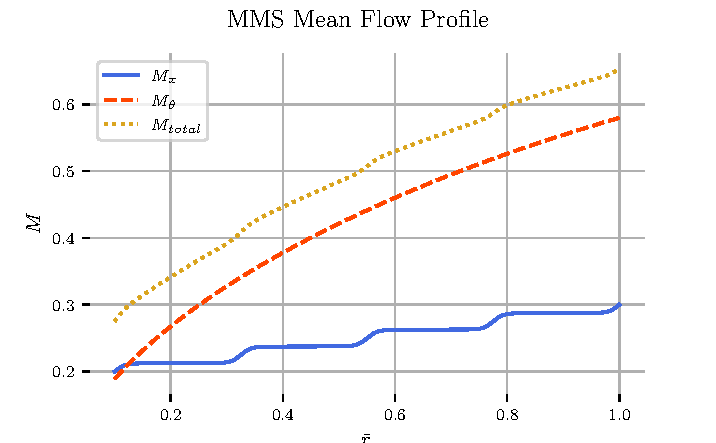
\includegraphics{/home/jeff-severino/SWIRL/CodeRun/03-plotReport/tex-outputs/MMS_mean_flow_profile.pdf}
    \caption{The manufactured mean flow test case using a summation of Tangents for $A$ and $M_x$}
    \label{fig:1}
\end{figure}


\begin{figure}[!]
    \centering
    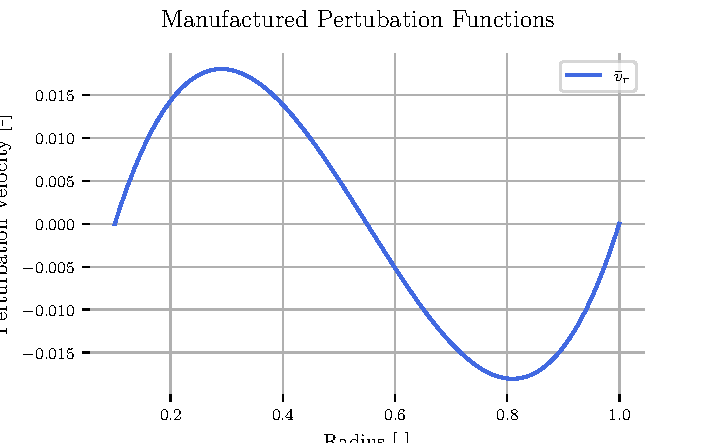
\includegraphics{/home/jeff-severino/SWIRL/CodeRun/03-plotReport/tex-outputs/MMS_perturbation_variables_vR.pdf}
\caption{The manufactured perturbation functions ,$v_r$}%, $v_x$, $v_{\theta}$, $p$}
    \label{fig:1a}
\end{figure}


\begin{figure}[!]
    \centering
    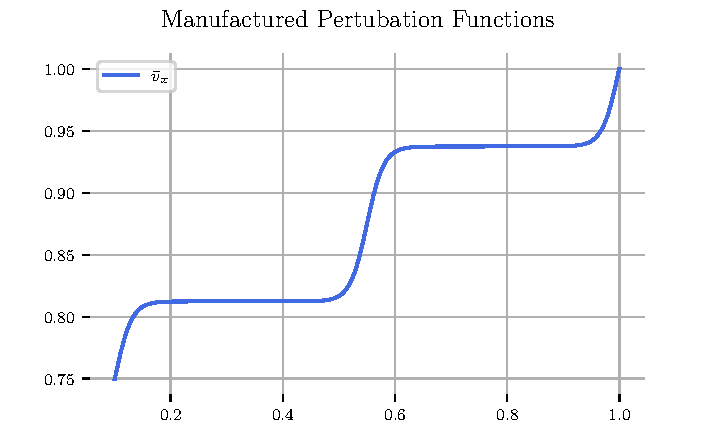
\includegraphics{/home/jeff-severino/SWIRL/CodeRun/03-plotReport/tex-outputs/MMS_perturbation_variables_vX.pdf}
\caption{The manufactured perturbation functions ,$v_x$}%, $v_x$, $v_{\theta}$, $p$}
    \label{fig:2a}
\end{figure}


\begin{figure}[!]
    \centering
    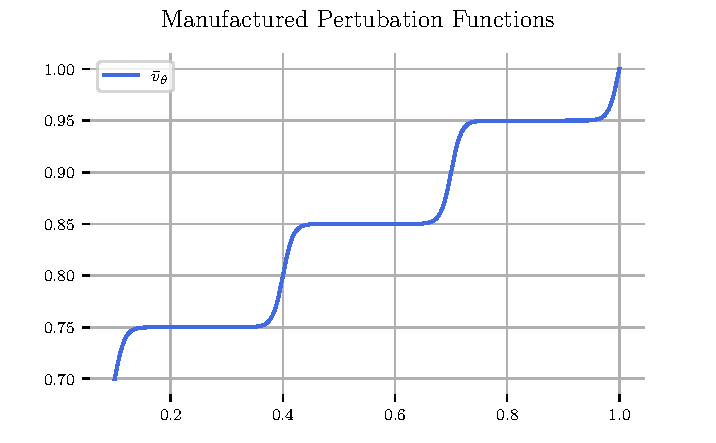
\includegraphics{/home/jeff-severino/SWIRL/CodeRun/03-plotReport/tex-outputs/MMS_perturbation_variables_vTh.pdf}
    \caption{The manufactured perturbation functions ,$v_{\theta}$}%, $v_x$, $v_{\theta}$, $p$}
    \label{fig:3a}
\end{figure}


\begin{figure}[!]
    \centering
    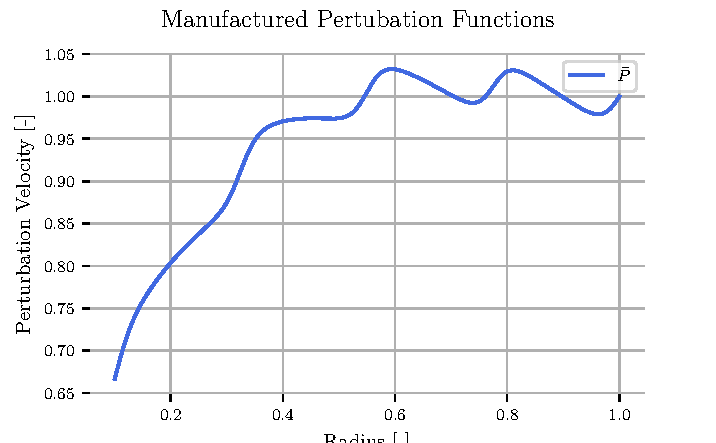
\includegraphics{/home/jeff-severino/SWIRL/CodeRun/03-plotReport/tex-outputs/MMS_perturbation_variables_Pr.pdf}
\caption{The manufactured perturbation functions ,$P$}%, $v_x$, $v_{\theta}$, $p$}
    \label{fig:4a}
\end{figure}

\begin{figure}[!]
    \centering
    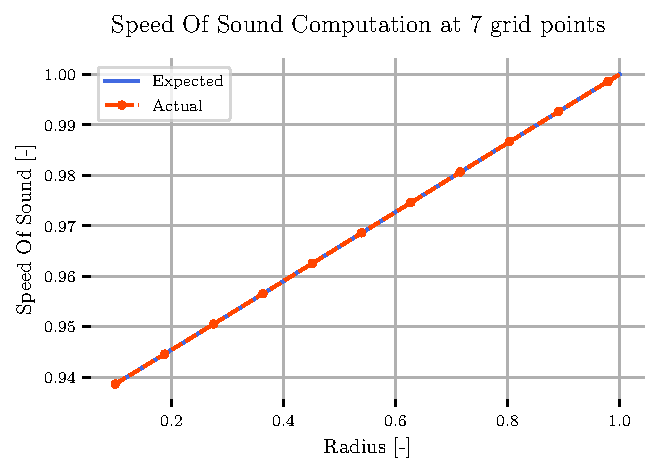
\includegraphics{/home/jeff-severino/SWIRL/CodeRun/03-plotReport/tex-outputs/SpeedOfSoundComparison1.pdf}
    \caption{ A comparison of the speed of sound, expected vs actual at the lowest grid to show similarities in solution}
    \label{fig:5}
\end{figure}


\begin{figure}[!]
    \centering
    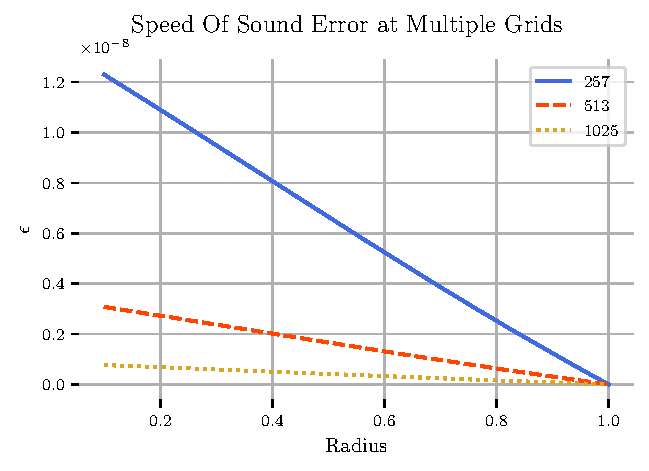
\includegraphics{/home/jeff-severino/SWIRL/CodeRun/03-plotReport/tex-outputs/SpeedOfSoundComparison2.pdf}
    \caption{ A comparison of the speed of sound error at three grid}
    \label{fig:5a}
\end{figure}


\begin{figure}[!]
    \centering
    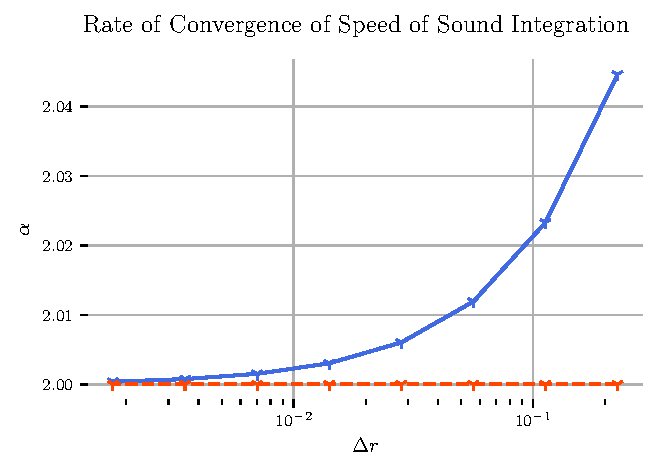
\includegraphics{/home/jeff-severino/SWIRL/CodeRun/03-plotReport/tex-outputs/SND_ROC.pdf}
    \caption{ A comparison of the speed of sound error at three grid}
    \label{fig:5a}
\end{figure}



\begin{figure}[!]
    \centering
    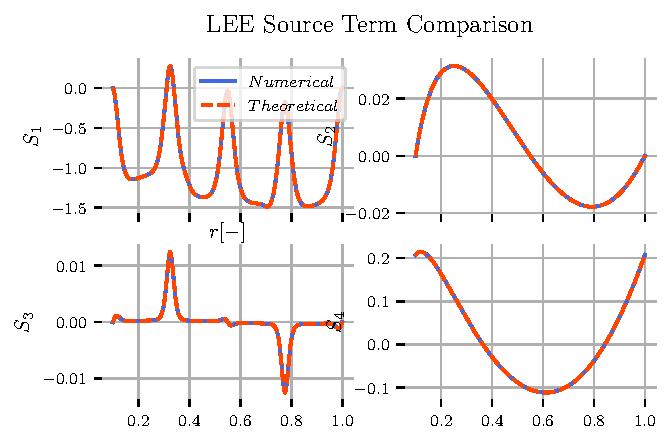
\includegraphics{/home/jeff-severino/SWIRL/CodeRun/03-plotReport/tex-outputs/SourceTermComparison.pdf}
    \caption{LEE Source Terms}
    \label{fig:6}
\end{figure}


\begin{figure}[!]
    \centering
    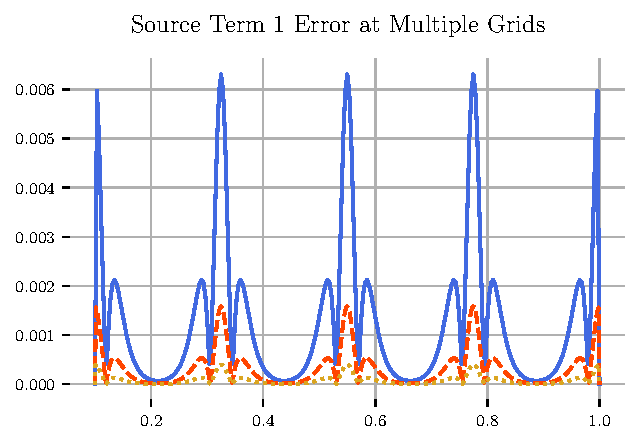
\includegraphics{/home/jeff-severino/SWIRL/CodeRun/03-plotReport/tex-outputs/SourceTermError1.pdf}
    \caption{LEE Source Term Error}
    \label{fig:7}
\end{figure}


\begin{figure}[!]
    \centering
    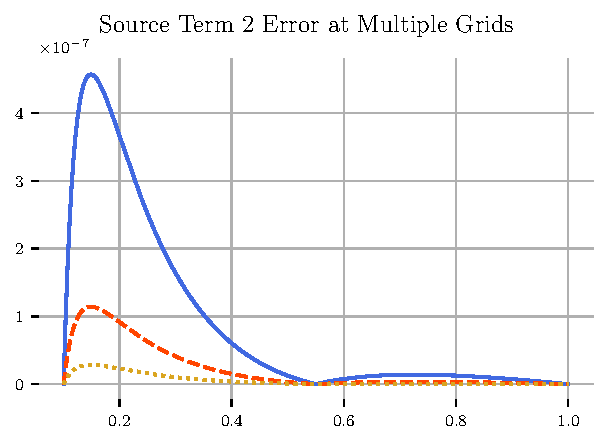
\includegraphics{/home/jeff-severino/SWIRL/CodeRun/03-plotReport/tex-outputs/SourceTermError2.pdf}
    \caption{LEE Source Term Error}
    \label{fig:7}
\end{figure}


\begin{figure}[!]
    \centering
    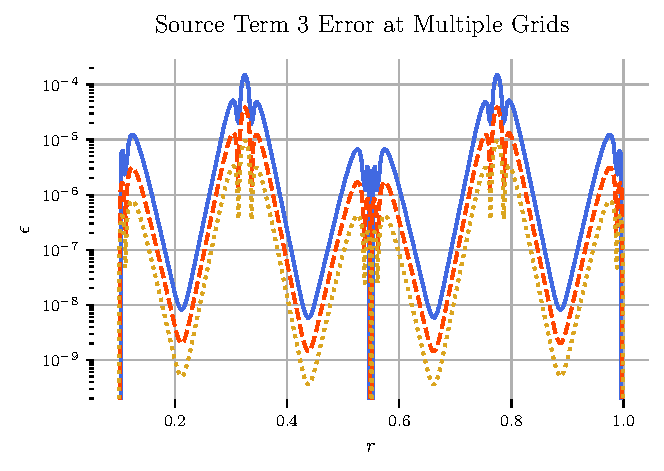
\includegraphics{/home/jeff-severino/SWIRL/CodeRun/03-plotReport/tex-outputs/SourceTermError3.pdf}
    \caption{LEE Source Term Error}
    \label{fig:7}
\end{figure}


\begin{figure}[!]
    \centering
    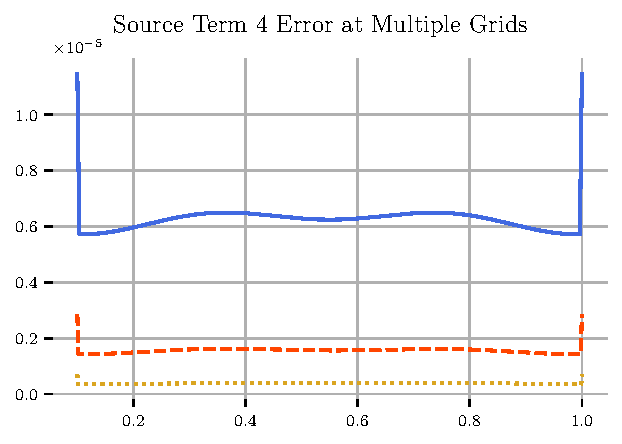
\includegraphics{/home/jeff-severino/SWIRL/CodeRun/03-plotReport/tex-outputs/SourceTermError4.pdf}
    \caption{LEE Source Term Error}
    \label{fig:7}
\end{figure}

\begin{figure}[!]
    \centering
    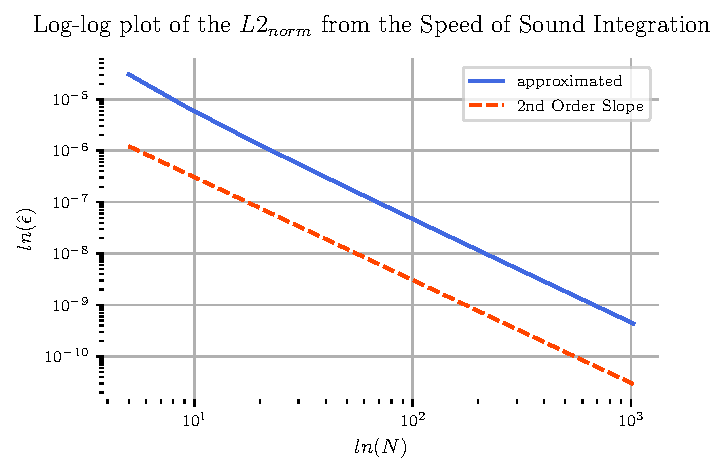
\includegraphics{/home/jeff-severino/SWIRL/CodeRun/03-plotReport/tex-outputs/SND_L2.pdf}
    \caption{L2 Norm comparison for the speed of sound integration for the compound trapezoidal rule}
    \label{fig:8}
\end{figure}



\begin{figure}[!]
    \centering
    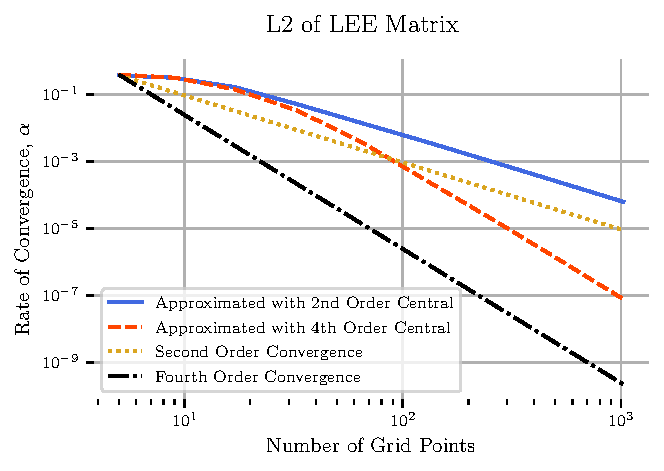
\includegraphics{/home/jeff-severino/SWIRL/CodeRun/03-plotReport/tex-outputs/LEE_L2.pdf}
    \caption{ROC  for the speed of sound integration for the compound trapezoidal rule}
    \label{fig:9}
\end{figure}


\begin{figure}[!]
    \centering
        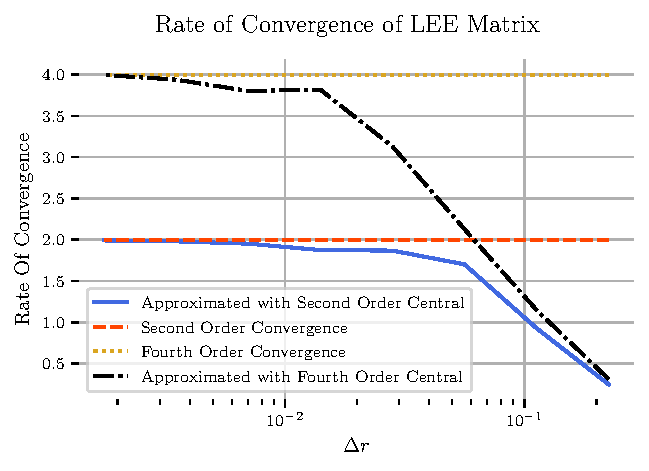
\includegraphics{/home/jeff-severino/SWIRL/CodeRun/03-plotReport/tex-outputs/LEE_ROC.pdf}
       \caption{ROC for the LEE using second and fourth order central differencing
       for the radial derivative}
        \label{fig:10}
\end{figure}





\section{Issues and Concerns}
- Need to change title in speed of sound comparison.
- Discuss the ROC for the second and fourth order schemes. 
- I would prefer to discuss the results separately.
\section{Planned Research}
Report MES. 
\end{document}


